% Left: the chord method on the unit circle. Right: the Markov tree. Generated by a short script.
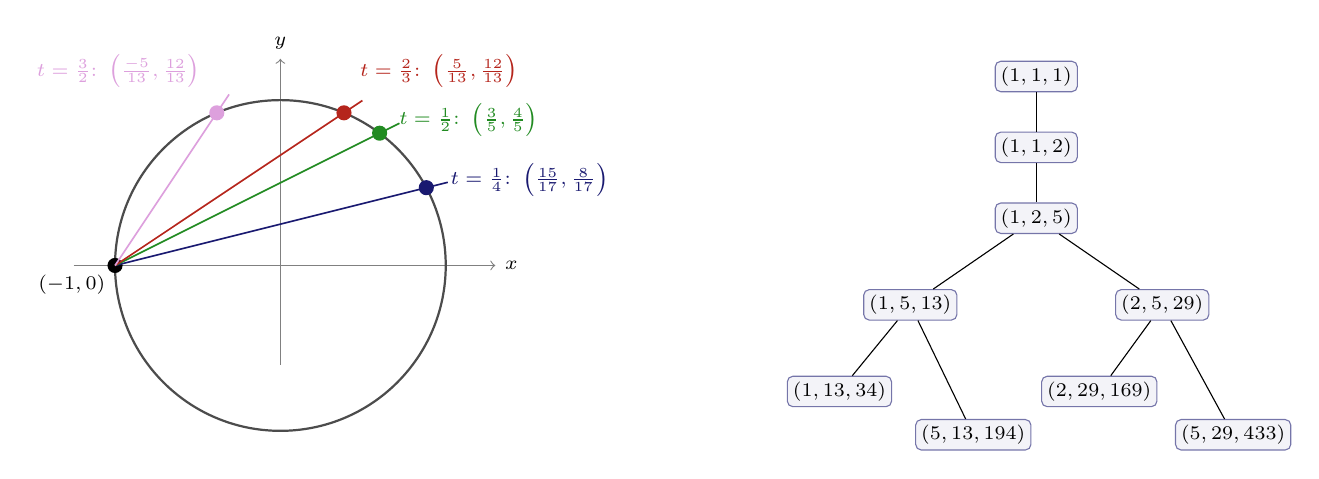
\begin{tikzpicture}
\begin{scope}[scale=2.1]
\draw[gray,->] (-1.25,0)--(1.3,0) node[right,font=\scriptsize,black] {$x$};
\draw[gray,->] (0,-0.6)--(0,1.25) node[above,font=\scriptsize,black] {$y$};
\draw[thick,black!70] (0,0) circle (1);
\fill (-1,0) circle (1.3pt) node[below left,font=\scriptsize] {$(-1,0)$};
\draw[MidnightBlue,semithick,shorten >=-8pt] (-1,0)--(0.8824,0.4706);
\fill[MidnightBlue] (0.8824,0.4706) circle (1.3pt);
\node[MidnightBlue,font=\scriptsize,anchor=west] at (0.9706,0.5176) {$t=\frac{1}{4}\colon\ \left(\frac{15}{17},\frac{8}{17}\right)$};
\draw[ForestGreen,semithick,shorten >=-8pt] (-1,0)--(0.6000,0.8000);
\fill[ForestGreen] (0.6000,0.8000) circle (1.3pt);
\node[ForestGreen,font=\scriptsize,anchor=west] at (0.6600,0.8800) {$t=\frac{1}{2}\colon\ \left(\frac{3}{5},\frac{4}{5}\right)$};
\draw[BrickRed,semithick,shorten >=-8pt] (-1,0)--(0.3846,0.9231);
\fill[BrickRed] (0.3846,0.9231) circle (1.3pt);
\node[BrickRed,font=\scriptsize,anchor=south west] at (0.4231,1.0154) {$t=\frac{2}{3}\colon\ \left(\frac{5}{13},\frac{12}{13}\right)$};
\draw[Plum,semithick,shorten >=-8pt] (-1,0)--(-0.3846,0.9231);
\fill[Plum] (-0.3846,0.9231) circle (1.3pt);
\node[Plum,font=\scriptsize,anchor=south east] at (-0.4231,1.0154) {$t=\frac{3}{2}\colon\ \left(\frac{-5}{13},\frac{12}{13}\right)$};
\end{scope}
\begin{scope}[xshift=9.6cm,yshift=2.4cm,every node/.style={font=\scriptsize,draw=MidnightBlue!60,fill=MidnightBlue!5,rounded corners=2pt,inner sep=2pt}]
\node (r) at (0,0) {$(1,1,1)$}; \node (a) at (0,-0.9) {$(1,1,2)$}; \node (b) at (0,-1.8) {$(1,2,5)$};
\node (c0) at (-1.6,-2.9) {$(1,5,13)$};
\draw (b)--(c0);
\node (c1) at (1.6,-2.9) {$(2,5,29)$};
\draw (b)--(c1);
\node (d0) at (-2.5,-4) {$(1,13,34)$};
\draw (c0)--(d0);
\node (d1) at (-0.8,-4.55) {$(5,13,194)$};
\draw (c0)--(d1);
\node (d2) at (0.8,-4) {$(2,29,169)$};
\draw (c1)--(d2);
\node (d3) at (2.5,-4.55) {$(5,29,433)$};
\draw (c1)--(d3);
\draw (r)--(a)--(b);
\end{scope}
\end{tikzpicture}
